\documentclass[usenames,dvipsnames,10pt,pdf,utf8,russian,aspectratio=43]{beamer}
\usepackage[english,russian]{babel}
\usepackage{cmap}
\usepackage[T2A]{fontenc}
\usepackage{subfig}
\usepackage{color}
\usepackage{tikz}
\usepackage{xargs}  
\usepackage{multicol}
\usepackage{amsmath}

%\usepackage{tikz,fullpage}
\DeclareMathOperator*{\argmax}{arg\,max}
\DeclareMathOperator*{\argmin}{arg\,min}

\usetikzlibrary{arrows,automata}
\usetikzlibrary{positioning}

%
% Choose how your presentation looks.
%
% For more themes, color themes and font themes, see:
% http://deic.uab.es/~iblanes/beamer_gallery/index_by_theme.html
%


\mode<presentation>
{


  \usetheme{Boadilla}      % or try Darmstadt, Madrid, Warsaw, ...
  \usecolortheme{seagull} % or try albatross, beaver, crane, ..

 \usefonttheme{structurebold}  % or try serif, structurebold, ...
  \setbeamertemplate{navigation symbols}{}
  \setbeamertemplate{caption}[numbered]
} 


\captionsetup[subfloat]{labelformat=empty}
\title[BP]{Bayesian programming}
\author{Бахтеев Олег}
\date{11.11.2020}

\begin{document}
% nb: очень не люблю макросы. Но что поделать 
% https://stackoverflow.com/questions/1509799/how-to-replace-latex-macros-with-their-definitions-using-latex
\newcommand{\D}{\mathfrak{D}}
\newcommand{\x}{\mathbf{x}}
\newcommand{\X}{\mathbf{X}}
\newcommand{\y}{\mathbf{y}}
\newcommand{\Xb}{\mathbb{X}}
\newcommand{\yb}{\mathbb{Y}}
\newcommand{\F}{\mathfrak{F}}



\newcommand{\w}{\mathbf{w}}
\newcommand{\Wb}{\mathbb{W}}
\newcommand{\Uw}{U_\mathbf{w}}

\newcommand{\Gam}{\boldsymbol{\Gamma}}
\newcommand{\Gb}{\amsmathbb{\Gamma}}
\newcommand{\UG}{U_{\boldsymbol{\Gamma}}}

\newcommand{\h}{\mathbf{h}}
\newcommand{\Hb}{\mathbb{H}}
\newcommand{\Uh}{U_{\mathbf{h}}}

\newcommand{\teta}{\boldsymbol{\theta}}
\newcommand{\Tetab}{\amsmathbb{\Theta}}
\newcommand{\Uteta}{U_{\boldsymbol{\theta}}}

\newcommand{\tetaw}{\boldsymbol{\theta}_\mathbf{w}}
\newcommand{\Tetawb}{\amsmathbb{\Theta}_\mathbf{w}}
\newcommand{\Utetaw}{U_{\boldsymbol{\theta}_\mathbf{w}}}
\newcommand{\tetaG}{\boldsymbol{\theta}_{\boldsymbol{\Gamma}}}
\newcommand{\TetaGb}{\amsmathbb{\Theta}_{\boldsymbol{\Gamma}}}
\newcommand{\UtetaG}{U_{\boldsymbol{\theta}_{\boldsymbol{\Gamma}}}}

\newcommand{\lam}{\boldsymbol{\lambda}}
\newcommand{\Lamb}{\amsmathbb{\Lambda}}
\newcommand{\Ulam}{U_{\boldsymbol{\lambda}}}

%\newcommand{\prior}{p(\mathbf{w}, \boldsymbol{\Gamma}|\mathbf{h},\boldsymbol{\lambda})}
\newcommandx{\prior}[4][1=\mathbf{w},2=\boldsymbol{\Gamma},3=\mathbf{h},4=\boldsymbol{\lambda},usedefault]{p(#1,#2|#3,#4)}
\newcommandx{\priorh}[2][1=\mathbf{h}, 2=\boldsymbol{\lambda},usedefault]{p(#1|#2)}
\newcommandx{\priorG}[3][1=\boldsymbol{\Gamma}, 2= \mathbf{h}, 3=\boldsymbol{\lambda},usedefault]{p(#1|#2,#3)}
\newcommandx{\priorw}[4][1=\mathbf{w},2=\boldsymbol{\Gamma},3=\mathbf{h},4=\boldsymbol{\lambda},usedefault]{p(#1|#2,#3,#4)}


\newcommand{\post}{p(\mathbf{w}, \boldsymbol{\Gamma}|\mathbf{y}, \mathbf{X}, \mathbf{h},\boldsymbol{\lambda})}
\newcommand{\posth}{p(\mathbf{h}|\mathbf{y}, \mathbf{X},\boldsymbol{\lambda})}
\newcommand{\postG}{p(\boldsymbol{\Gamma}|\mathbf{y}, \mathbf{X}, \mathbf{h},\boldsymbol{\lambda})}
\newcommand{\postw}{p(\mathbf{w}|\mathbf{y}, \mathbf{X}, \boldsymbol{\Gamma}, \mathbf{h},\boldsymbol{\lambda})}


\newcommandx{\q}[1][1=\boldsymbol{\theta}, usedefault]{q(\mathbf{w}, \boldsymbol{\Gamma}|#1)}
\newcommandx{\qG}[2][1=\boldsymbol{\Gamma},2=\boldsymbol{\theta}_{\boldsymbol{\Gamma}},usedefault]{q_{\boldsymbol{\Gamma}}(#1|#2)}
\newcommandx{\qw}[3][1=\mathbf{w}, 2=\boldsymbol{\Gamma},3=\boldsymbol{\theta}_\mathbf{w},usedefault]{q_\mathbf{w}(#1|#2,#3)}


\newcommandx{\LL}[4][1=\mathbf{y},2=\mathbf{X},3=\mathbf{w},4=\boldsymbol{\Gamma},usedefault]{p(#1|#2,#3,#4)}

\newcommand{\EV}{p(\mathbf{y}|\mathbf{X}, \mathbf{h},\boldsymbol{\lambda})}

\newcommandx{\Loss}[5][1=\boldsymbol{\theta},2=\mathbf{y},3=\mathbf{X},4=\mathbf{h},5=\boldsymbol{\lambda},usedefault]{L(#1 |#2,#3,#4,#5)}
\newcommandx{\Val}[5][1=\mathbf{h},2=\mathbf{y},3=\mathbf{X},4=\boldsymbol{\theta},5=\boldsymbol{\lambda},usedefault]{Q(#1|#2,#3,#4,#5)}

% прочее
\newcommand{\model}{\mathbf{f}}
\newcommand{\A}{\mathbf{A}}
\newcommand{\s}{\mathbf{s}}
\newcommand{\g}{\boldsymbol{\gamma}}
\newcommand{\E}{\mathsf{E}}
\newcommand{\KL}[2]{D_\text{KL}\bigl(#1 || #2\bigr)}

\newcommand{\lamT}{\lambda_{\text{temp}}}
\newcommand{\lamLL}{\lambda_\text{likelihood}^\text{Q}}
\newcommand{\lamCL}{\lambda_\text{prior}^\text{L}}
\newcommand{\lamCQ}{\lambda_\text{prior}^\text{Q}}
\newcommand{\lamS}{\boldsymbol{\lambda}_\text{struct}^\text{Q}}
\newcommandx{\TLoss}[6][1=\boldsymbol{\theta},2=L,3=\mathbf{y}, 4=\mathbf{X}, 5=\mathbf{h},6=\boldsymbol{\lambda},usedefault]{T(#1|#2,#3,#4,#5,#6)}
\newcommandx{\TVal}[6][1=\mathbf{h},2=Q,3=\mathbf{y}, 4=\mathbf{X}, 5=\boldsymbol{\teta},6=\boldsymbol{\lambda},usedefault]{T(#1|#2,#3,#4,#5,#6)}
%\newcommand{\log}{\text{log}~}




\begin{frame}
  \titlepage
\end{frame}

\begin{frame}{Мотивация}
Любой предмет представляется человеку как совокупность связанных между собой понятий.
\centering
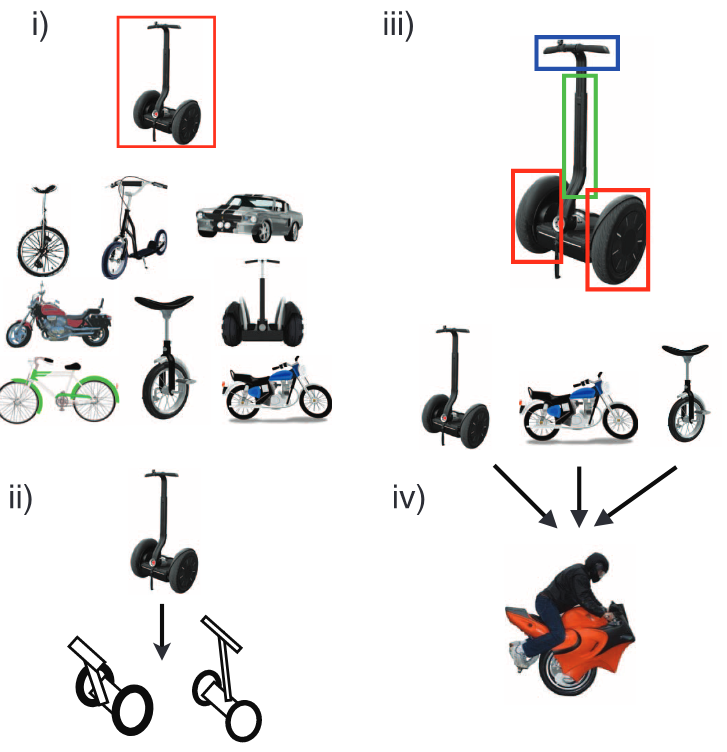
\includegraphics[width=0.5\textwidth]{moto.png}
\end{frame}

\begin{frame}{Основные работы}
\begin{itemize}
\item Lake B. M., Salakhutdinov R., Tenenbaum J. B. Human-level concept learning through probabilistic program induction //Science. – 2015. – Т. 350. – №. 6266. – С. 1332-1338.
\item Lake B. M. et al. Building machines that learn and think like people //Behavioral and brain sciences. – 2017. – Т. 40.
\item Lake B. M., Salakhutdinov R. R., Tenenbaum J. One-shot learning by inverting a compositional causal process //Advances in neural information processing systems. – 2013. – С. 2526-2534.
\end{itemize}
\end{frame}

\begin{frame}{Постановка}
\begin{block}{One-shot classification}
 The tasks tested within-alphabet classification on 10 alphabets.  Each trial (of 400 total) consists of a single test image ofa new character compared to 20 new characters from the same alphabet, given just one image eachproduced by a typical drawer of that alphabet.
\end{block}
\centering
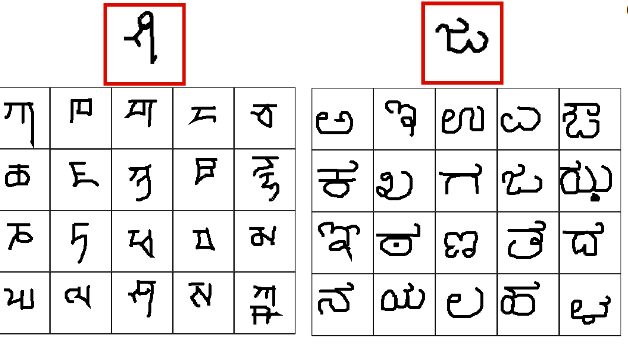
\includegraphics[width=0.5\textwidth]{omni.png}
\end{frame}


\begin{frame}{Идея подхода}
\textbf{Три ключевые концепции подхода}
\begin{itemize}
\item Композиционность
\begin{itemize}
\item Объект разбивается на несколько элементов
\item Каждый элемент характеризуется своей генеративной моделью
\end{itemize}

\item Причинность
\begin{itemize}
\item Над элементами вводится вероятностная иерархия
\item Элемент сам по себе представляется в иерархическом виде (токен и тип токена)
\end{itemize}

\item Обучение обучению
\begin{itemize}
\item Настройка гиперпараметров на обучающем датасете 
\end{itemize}


\end{itemize}
\end{frame}

\begin{frame}{Модель}
\centering
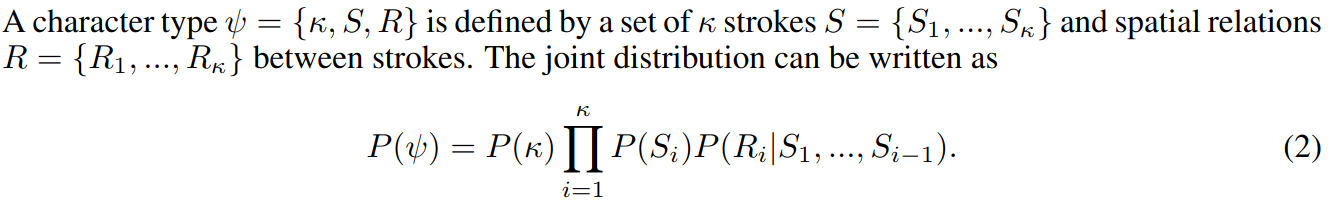
\includegraphics[width=0.75\textwidth]{bp1.png}
\centering
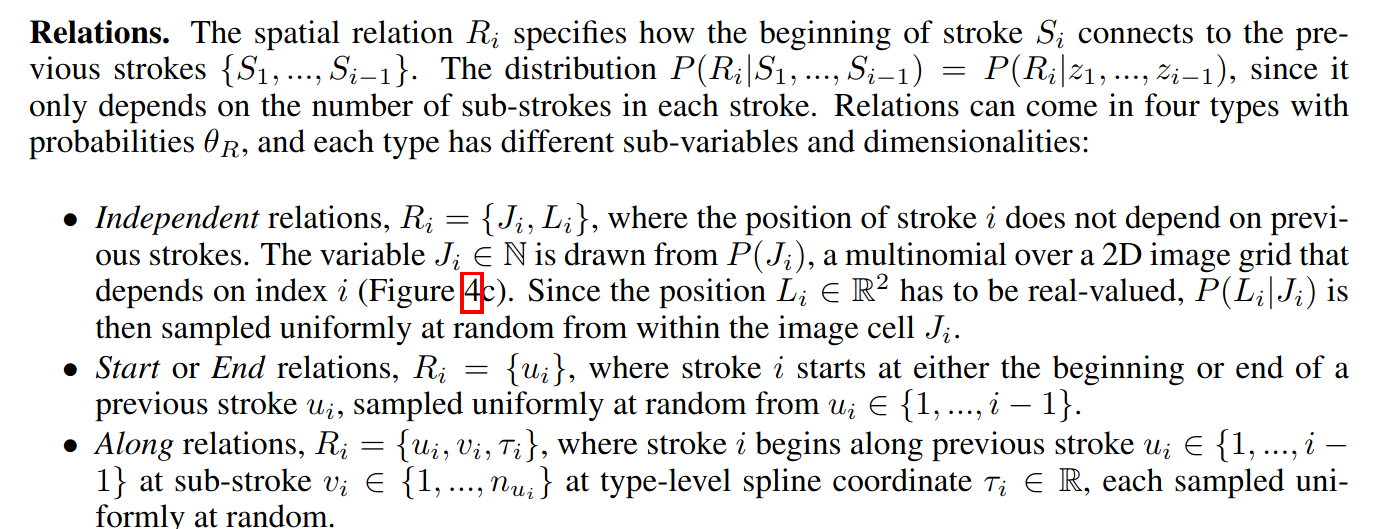
\includegraphics[width=0.75\textwidth]{bp2.png}
\centering
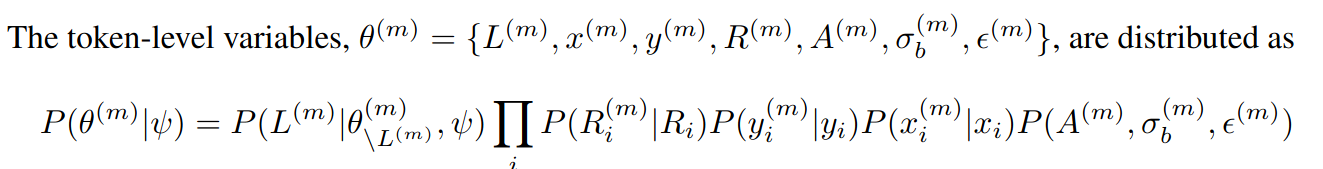
\includegraphics[width=0.75\textwidth]{bp3.png}

\end{frame}

\begin{frame}{Модель}
\centering
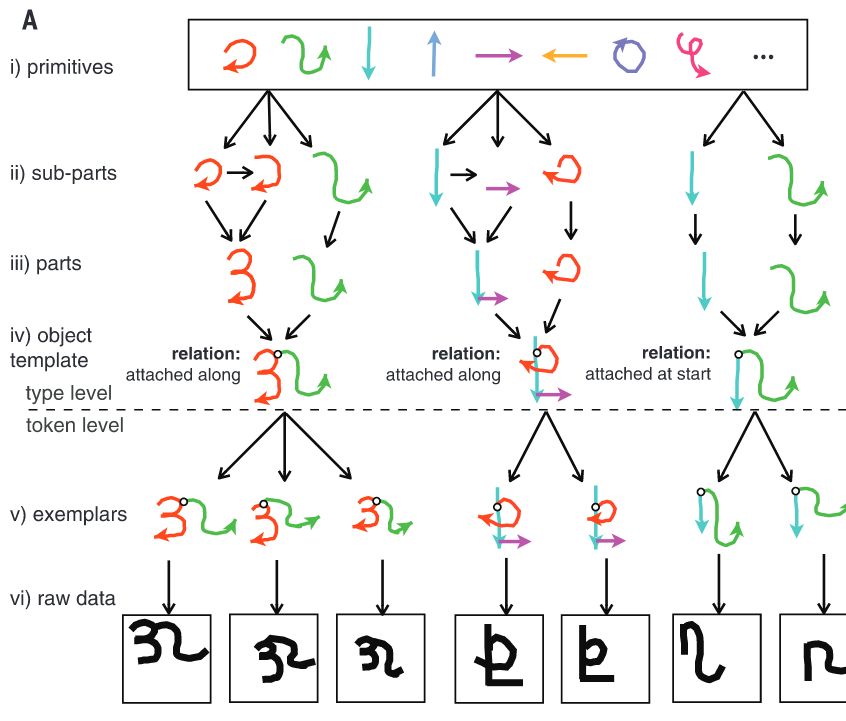
\includegraphics[width=0.75\textwidth]{bp4a.png}

\end{frame}


\begin{frame}{Результат}
\centering
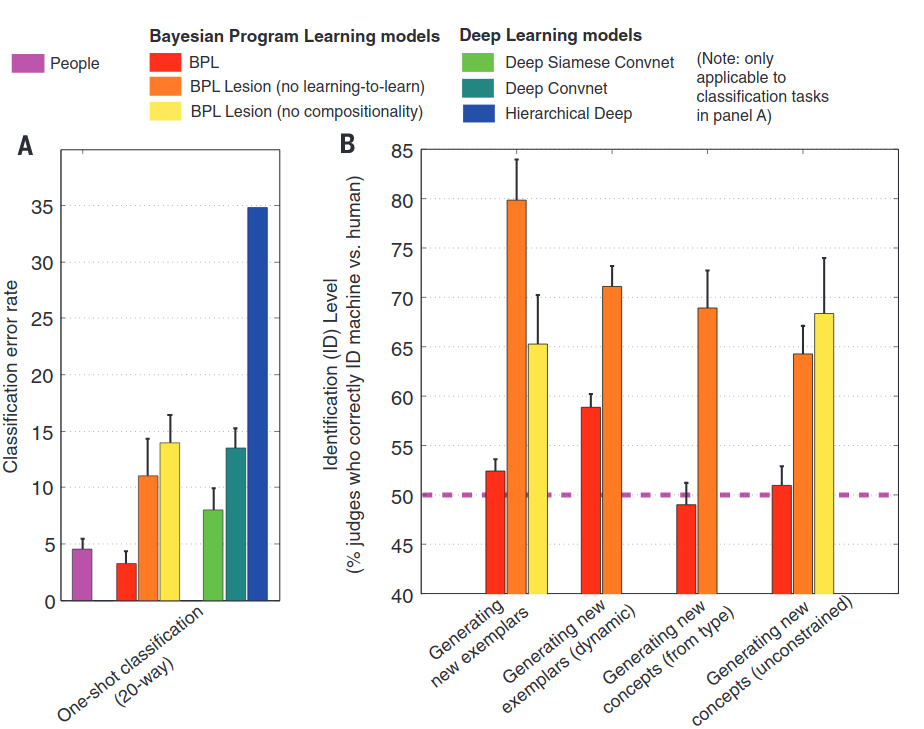
\includegraphics[width=0.75\textwidth]{bp6.png}

\end{frame}





\begin{frame}{Идея подхода}
\textbf{Где нашли продолжение описанные концепции?}
\begin{itemize}
\item Композиционность
\item Причинность
\item Обучение обучению
\end{itemize}
\end{frame}





\begin{frame}{Идея подхода}
\textbf{Где нашли продолжение описанные концепции?}
\begin{itemize}
\item Композиционность

\item Причинность
\begin{itemize}
\item Attention и Self-attention
\item Иерархические генеративные модели и смеси
\end{itemize}
\item Обучение обучению
\end{itemize}
\end{frame}


\begin{frame}{Работа с разными модальностями}
\centering

\centering
\begin{figure}
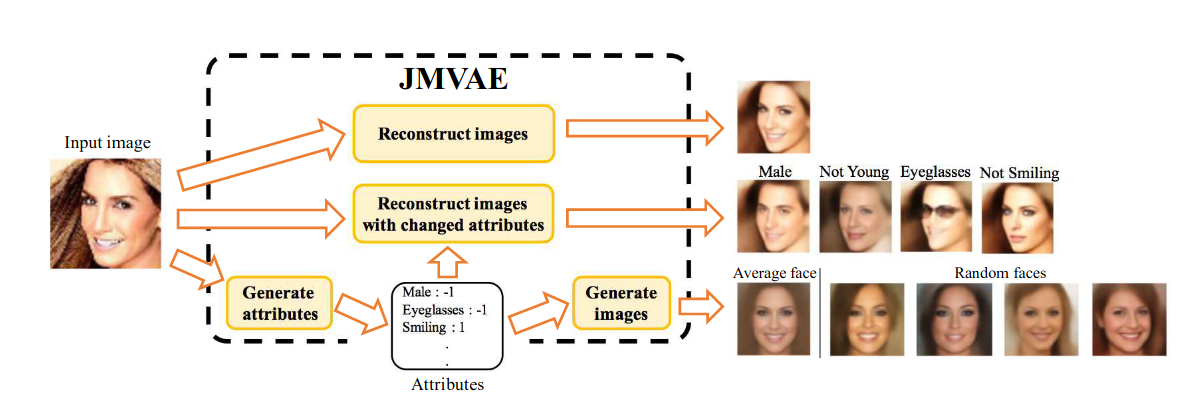
\includegraphics[width=0.6\textwidth]{jmvae.png}
\caption{Suzuki et al., 2017 }
\end{figure}

\begin{figure}
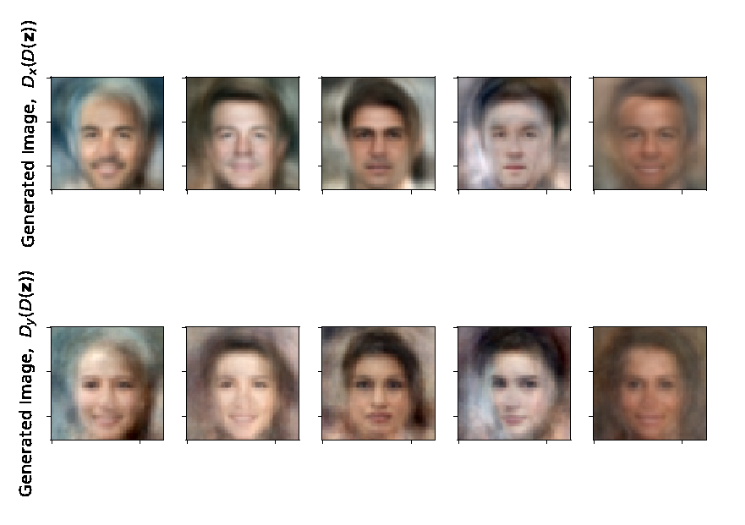
\includegraphics[width=0.35\textwidth]{vbta.png}
\caption{Kuznetsova et al., 2018}
\end{figure}


\end{frame}



\begin{frame}{Метапараметры}
\begin{block}{Wikipedia}
A parameter that controls the value of one or more others.
\end{block}

\begin{block}{Определение}
Метапараметрами $\boldsymbol{\lambda}$ модели назовем параметры оптимизации.
\end{block}

Чаще всего метапараметры назначаются экспертно и не подлежат оптимизации в ходе решения задачи выбора модели. 

Что можно считать метапараметрами:
\begin{itemize}
\item параметры оператора оптимизации;
\item параметры задачи оптимизации;
\item структуру модели;
\item функции активации слоев сети;
\item вид априорного распределения и функции правдоподобия.
\end{itemize}
\end{frame}


\begin{frame}{A neural network that embeds its own meta-levels}
Предлагается разделить подмодели внутри модели сети по назначениям:
\begin{itemize}
\item ``Normal'' model: обучение и вывод.
\item Evaluation model: оценка качества $Q$.
\item Analyzing model: анализ параметров модели.
\item Modifiyng model: модификация параметров.
\end{itemize}

Представлен градиентный алгоритм оптимизации нейронной сети.
\end{frame}



\begin{frame}{L2L by gradient descent by gradient descent}

\textbf{Идея: } рассматривать результат применения градиентного спуска $T$ как дифференцируемую функцию:
\[
    T(\boldsymbol{\theta}) = \text{LSTM}(\boldsymbol{\theta}).
\]
Оптимизационная задача:
\[
    \sum_{t=t_0}^{t_\eta} L\left(T^t(\boldsymbol{\theta}_{t_0})\right) \to \min.
\]

LSTM имеет небольшое число параметров и делит параметры между всеми параметрами, подлежащими оптимизации.

\begin{figure}
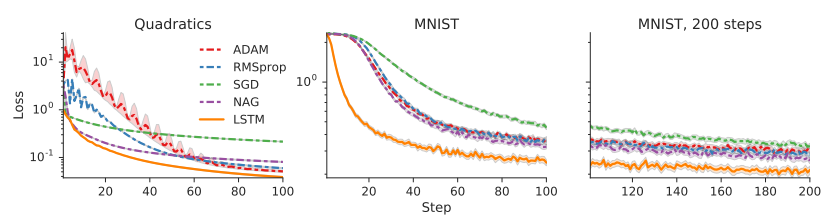
\includegraphics[width=\textwidth]{sgd_by_sgd.png}
\end{figure}
\end{frame}


\begin{frame}
\frametitle{Список источников}
\begin{itemize}
\item Lake B. M., Salakhutdinov R., Tenenbaum J. B. Human-level concept learning through probabilistic program induction //Science. – 2015. – Т. 350. – №. 6266. – С. 1332-1338.
\item Lake B. M. et al. Building machines that learn and think like people //Behavioral and brain sciences. – 2017. – Т. 40.
\item Lake B. M., Salakhutdinov R. R., Tenenbaum J. One-shot learning by inverting a compositional causal process //Advances in neural information processing systems. – 2013. – С. 2526-2534.
\item Suzuki M., Nakayama K., Matsuo Y. Joint multimodal learning with deep generative models //arXiv preprint arXiv:1611.01891. – 2016.
\item Kuznetsova R., Bakhteev O., Ogaltsov A. Variational learning across domains with triplet information //arXiv preprint arXiv:1806.08672. – 2018.
\item Schmidhuber J. A neural network that embeds its own meta-levels //IEEE International Conference on Neural Networks. – IEEE, 1993. – С. 407-412.
\item Andrychowicz M. et al. Learning to learn by gradient descent by gradient descent //Advances in neural information processing systems. – 2016. – С. 3981-3989.
\end{itemize}
\end{frame}


\end{document}

